% !TEX root = ../../../main.tex
% 来源：中学数学实验教材·第一册（代数）
% 章节：因式分解与余式定理 / 辗转相除法
% 原始文件：5.tex，行 2946-2971
% 类型：tikz
% ---
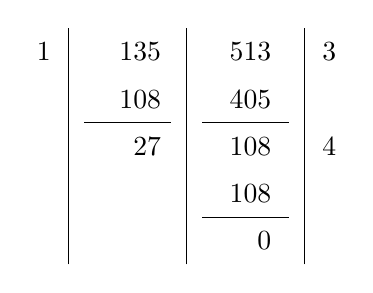
\begin{tikzpicture}[yscale=.6]
\foreach \x/\xtext in {6/135, 5/108, 4/\boxed{27}}
{
    \node at (-.2,\x)[left]{$\xtext$};
}

\foreach \x/\xtext in {6/513, 5/405, 4/108, 3/108, 2/0}
{
    \node at (1.2,\x)[left]{$\xtext$};
}

\foreach \x in {0,-1.5,1.5}
{
    \draw (\x, 1.5)--(\x, 6.5);
}

\draw (-1.3, 4.5)--(-0.2, 4.5);
\draw (0.2, 4.5)--(1.3,4.5);
\draw (0.2, 2.5)--(1.3,2.5);


\node at (-1.6,6)[left]{1};
\node at (1.6,6)[right]{3};
\node at (1.6,4)[right]{4};

\end{tikzpicture}    
